\chapter{The COMET Experiment}\label{ch:comet}

% \begin{markdown}
% ---

% - Description of the COMET experiment's goal, design with nice illustrations
%     + Signal and background:
%         + mu-e conv signal description
%         + **List of background sources**
% + CyDet:
%     + For simulation section, need to explain how CDC and CTH work, and how
%       combined they enable mu--e conv measurement
%     - Detailed description of the CDC, which is crucial for the GAN section.
%      - Stereo angles
% + Phase alpha?

% - References: TDR, SINDRUM II, 

% ---

% + Requirements: high sensitivity to signal, efficient rejection of backgrounds
%  + -> Need intense muon beam, pulsed, and detector design must avoid
%    backgrounds
% + TIMING of signal (muon lifetime)
% + Proton beam energy: why 8 Gev -> antiproton production
% + Intensity: beam current, beam power, POTs per second
% + Send backward-going secondaries to detector, discard the main part of
%   secondaries (forward-going)
% + Curved solenoid + dipole field (by tilting coils, see Krikler)
% + Stopping target -> why Al
% + Bunch structure, extinction
% + Phase-I detectors: StrECAL and CyDet

% ---
% \end{markdown}

% Description and goals
COMET (COherent Muon to Electron Transition) is a future muon-beam experiment
designed to search for the muon to electron conversion
process~\cite{the_comet_collaboration_comet_2020}. It is currently under
construction at the Japan Proton Accelerator Research Complex (J-PARC) facility
in Tokai, Japan. The goal of COMET is to be \numprint{10000} times more
sensitive to $\mu$--$e$ conversion than the current world-leading limit set by
the SINDRUM II experiment~\cite{Bertl:2006up}. 

\subsubsection{Requirements}
In order to reach its goal, the COMET experiment is designed with strict
requirements defined to make the conversion signal as clear as possible, while
efficiently rejecting background events. The essential requirements that define
the COMET experiment are:
\begin{itemize}
    \item An intense muon source to probe the rare conversion process;
    \item A pulsed beam such that timing information can be used to reject
    backgrounds;
    \item Strict selection of charge and momentum of beam particles prior to
    reaching the detector;
    \item A tracking detector to search for the \SI{104.97}{\MeV} conversion
    signature.
\end{itemize}
These requirements and the design choices that were made to address them are
described in more detail in the rest of this chapter.

\subsubsection{Strategy}
COMET is planned to run in a staged approach such that the properties of the
newly designed beam can be finely understood before making the measurement.
COMET Phase-I has a double purpose, each fulfilled by a distinct detector
system. The StrECAL detector, composed of a straw-tube tracker and
electromagnetic calorimeter, will study the beam composition and timing
properties and increase our understanding of potential backgrounds. The
Cylindrical Detector, composed of a cylindrical drift chamber and a trigger
hodoscope, will be used to perform a $\mu$--$e$ conversion search with a
single-event sensitivity (see Section~\ref{sec:SES}) of $3\times 10^{-15}$, a
factor-100 improvement over SINDRUM II. COMET Phase-II is a planned upgrade to
Phase-I with higher beam intensity and better background rejection via a longer
momentum-selecting beamline. Phase-II aims to improve on the single-event
sensitivity of Phase-I by another factor $100$ to reach a single event
sensitivity of $2.6\times 10^{-17}$.

\subsubsection{Design}
Figure~\ref{fig:comet_schematic} shows a top-down schematic view of the COMET
experiment, laying out the different sections that make up the beamline in
Phase-I and Phase-II. In the latter, the transport solenoid is doubled to allow
more pions to decay into muons while tightening the momentum selection further.
An additional curved solenoid, the \emph{electron spectrometer,} further
eliminates particles whose momenta do not match the \SI{104.97}{\MeV} conversion
signature before they enter the detector system. While Phase-I will use the
StrECAL to study the beam properties, Phase-II will use it as the
conversion-searching detector system.\\
The following sections describe in more detail each component of the COMET
beamline.

\begin{figure}
    \centering
    \begin{subfigure}[b]{0.46\textwidth}
    \centering
        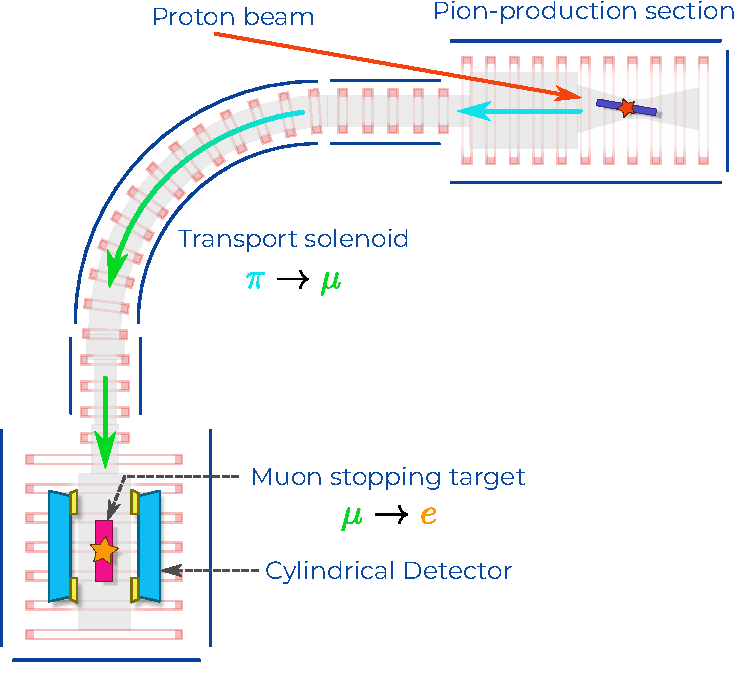
\includegraphics[width=\textwidth]{chapter2/comet_schematic_phase-I.pdf}
        \vspace{3cm}
        \caption{Phase-I with the Cylindrical Detector.}
    \end{subfigure}
    \hfill
    \begin{subfigure}[b]{0.49\textwidth}
        \centering
        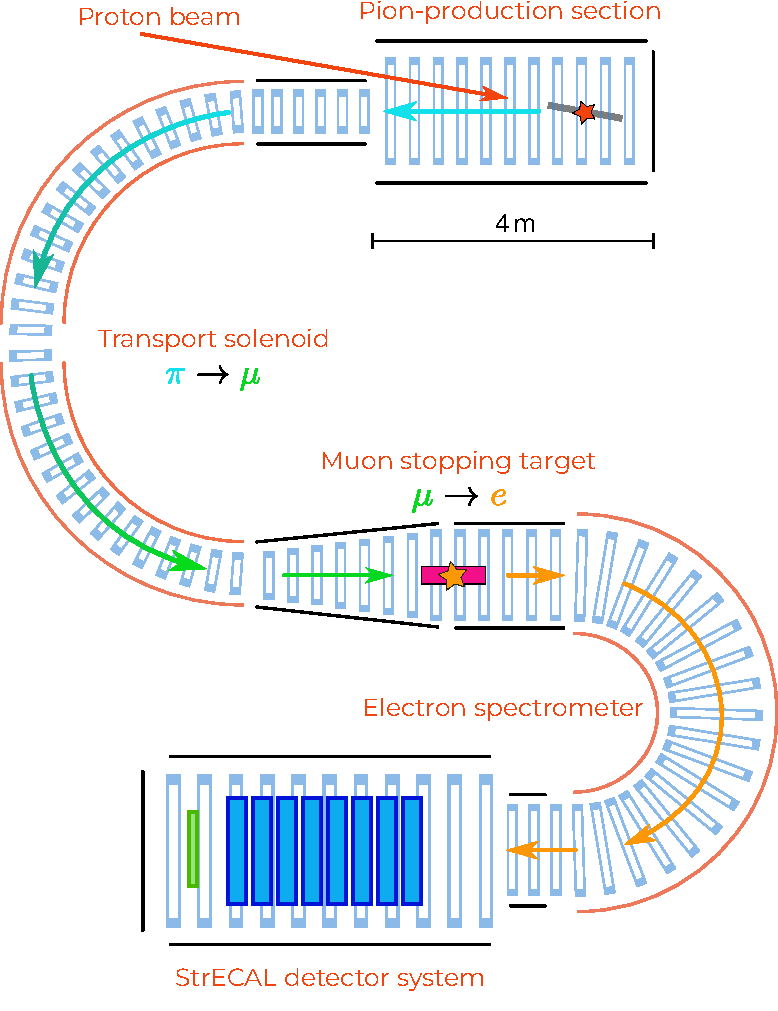
\includegraphics[width=\textwidth]{chapter2/comet_schematic.pdf}
        \caption{Phase-II.}
    \end{subfigure}
    \caption{ Schematic top-down view of the COMET experiment. The beam pipe is
    represented in grey, and the light red rectangles along the beamline
    represent the solenoids that generate the magnetic field. Curved solenoids
    additionally help to select charge and momentum, as discussed in
    Section~\ref{sec:curved_solenoids}.}
    \label{fig:comet_schematic}
\end{figure}



\section{Proton beam}\label{sec:COMET_beam}

Muons in the COMET experiment are produced from the decay of pions created in
proton collisions on a static solid target. The primary proton beam is provided
by the J-PARC facility. Protons are delivered with an energy of \SI{8}{\GeV},
which is picked to maximise the pion yield while minimising the production of
anti-protons, a potential background source.

The timeline of a COMET event is shown in Figure~\ref{fig:timing_distributions}.
The beam has a pulsed time profile: protons are grouped into \SI{100}{\ns}
bunches, each containing $16\times 10^6$ protons. Bunches are separated by
\SI{1170}{\ns}. Just after the collision, secondary particles will quickly move
down the COMET beamline and produce numerous background hits in the detector
system. This prompt and intense flooding of the detector is called the
\emph{beam flash}, and typically dies down within a few hundred nanoseconds.
Muons bound by the muon stopping target have a lifetime of \SI{864}{\ns} (see
Section~\ref{sec:stopping_target}). This, combined with the \SI{1170}{\ns} time
span between two bunches, allows COMET to search for $\mu$--$e$ conversion after
the beam flash has ended, and until the next collision occurs. 

\begin{figure}
    \centering
    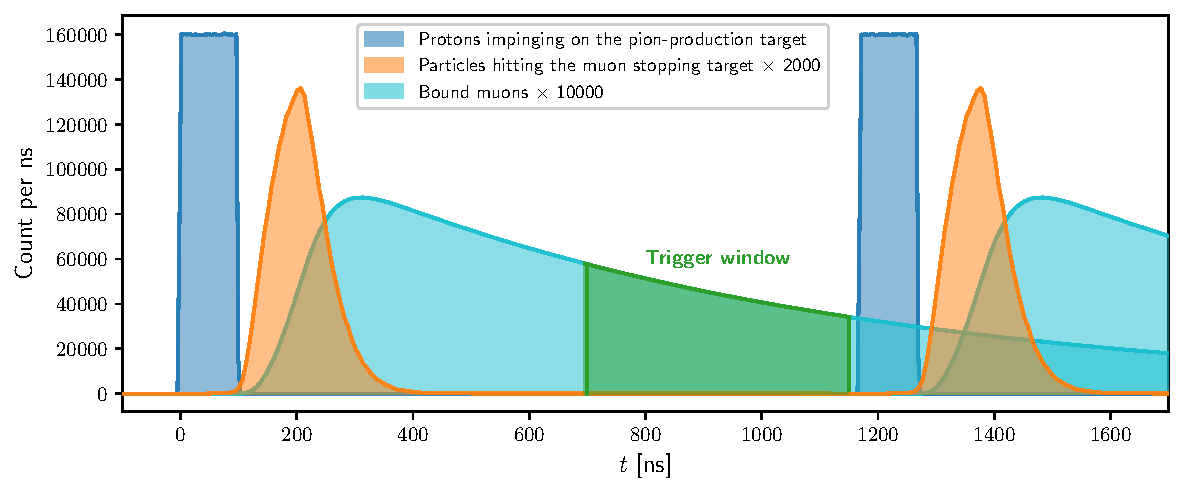
\includegraphics[width=0.85\textwidth]{chapter2/timing_plot_realistic_beam_flash.pdf}
    \caption{ Timeline of a COMET event. Shortly after the proton collision, the
        beam flash floods the detector and muons begin to be bound in the muon
        stopping target. The Phase-I trigger window shown here starts at
        $t=\SI{700}{\ns}$ and lasts until the next proton bunch collision.  }
    \label{fig:timing_distributions}
\end{figure}

% Could also add info on buckets, 4/5 time structure

Stray protons arriving in the time between two bunches can contribute to the
experimental backgrounds by sending particles toward the detector region at
unexpected timings. COMET requires the J-PARC proton beam to have fewer than one
such stray proton for every 600 bunches in order to reach its sensitivity goals.
This corresponds to an extinction factor
\begin{equation}\label{eq:extinction}
R_\mathrm{extinction} \equiv \frac{\mathrm{protons\ between\
bunches}}{\mathrm{protons\ per\ bunch}} \approx 10^{-10}.
\end{equation}

\section{Pion-production section}

\begin{figure}
    \centering
    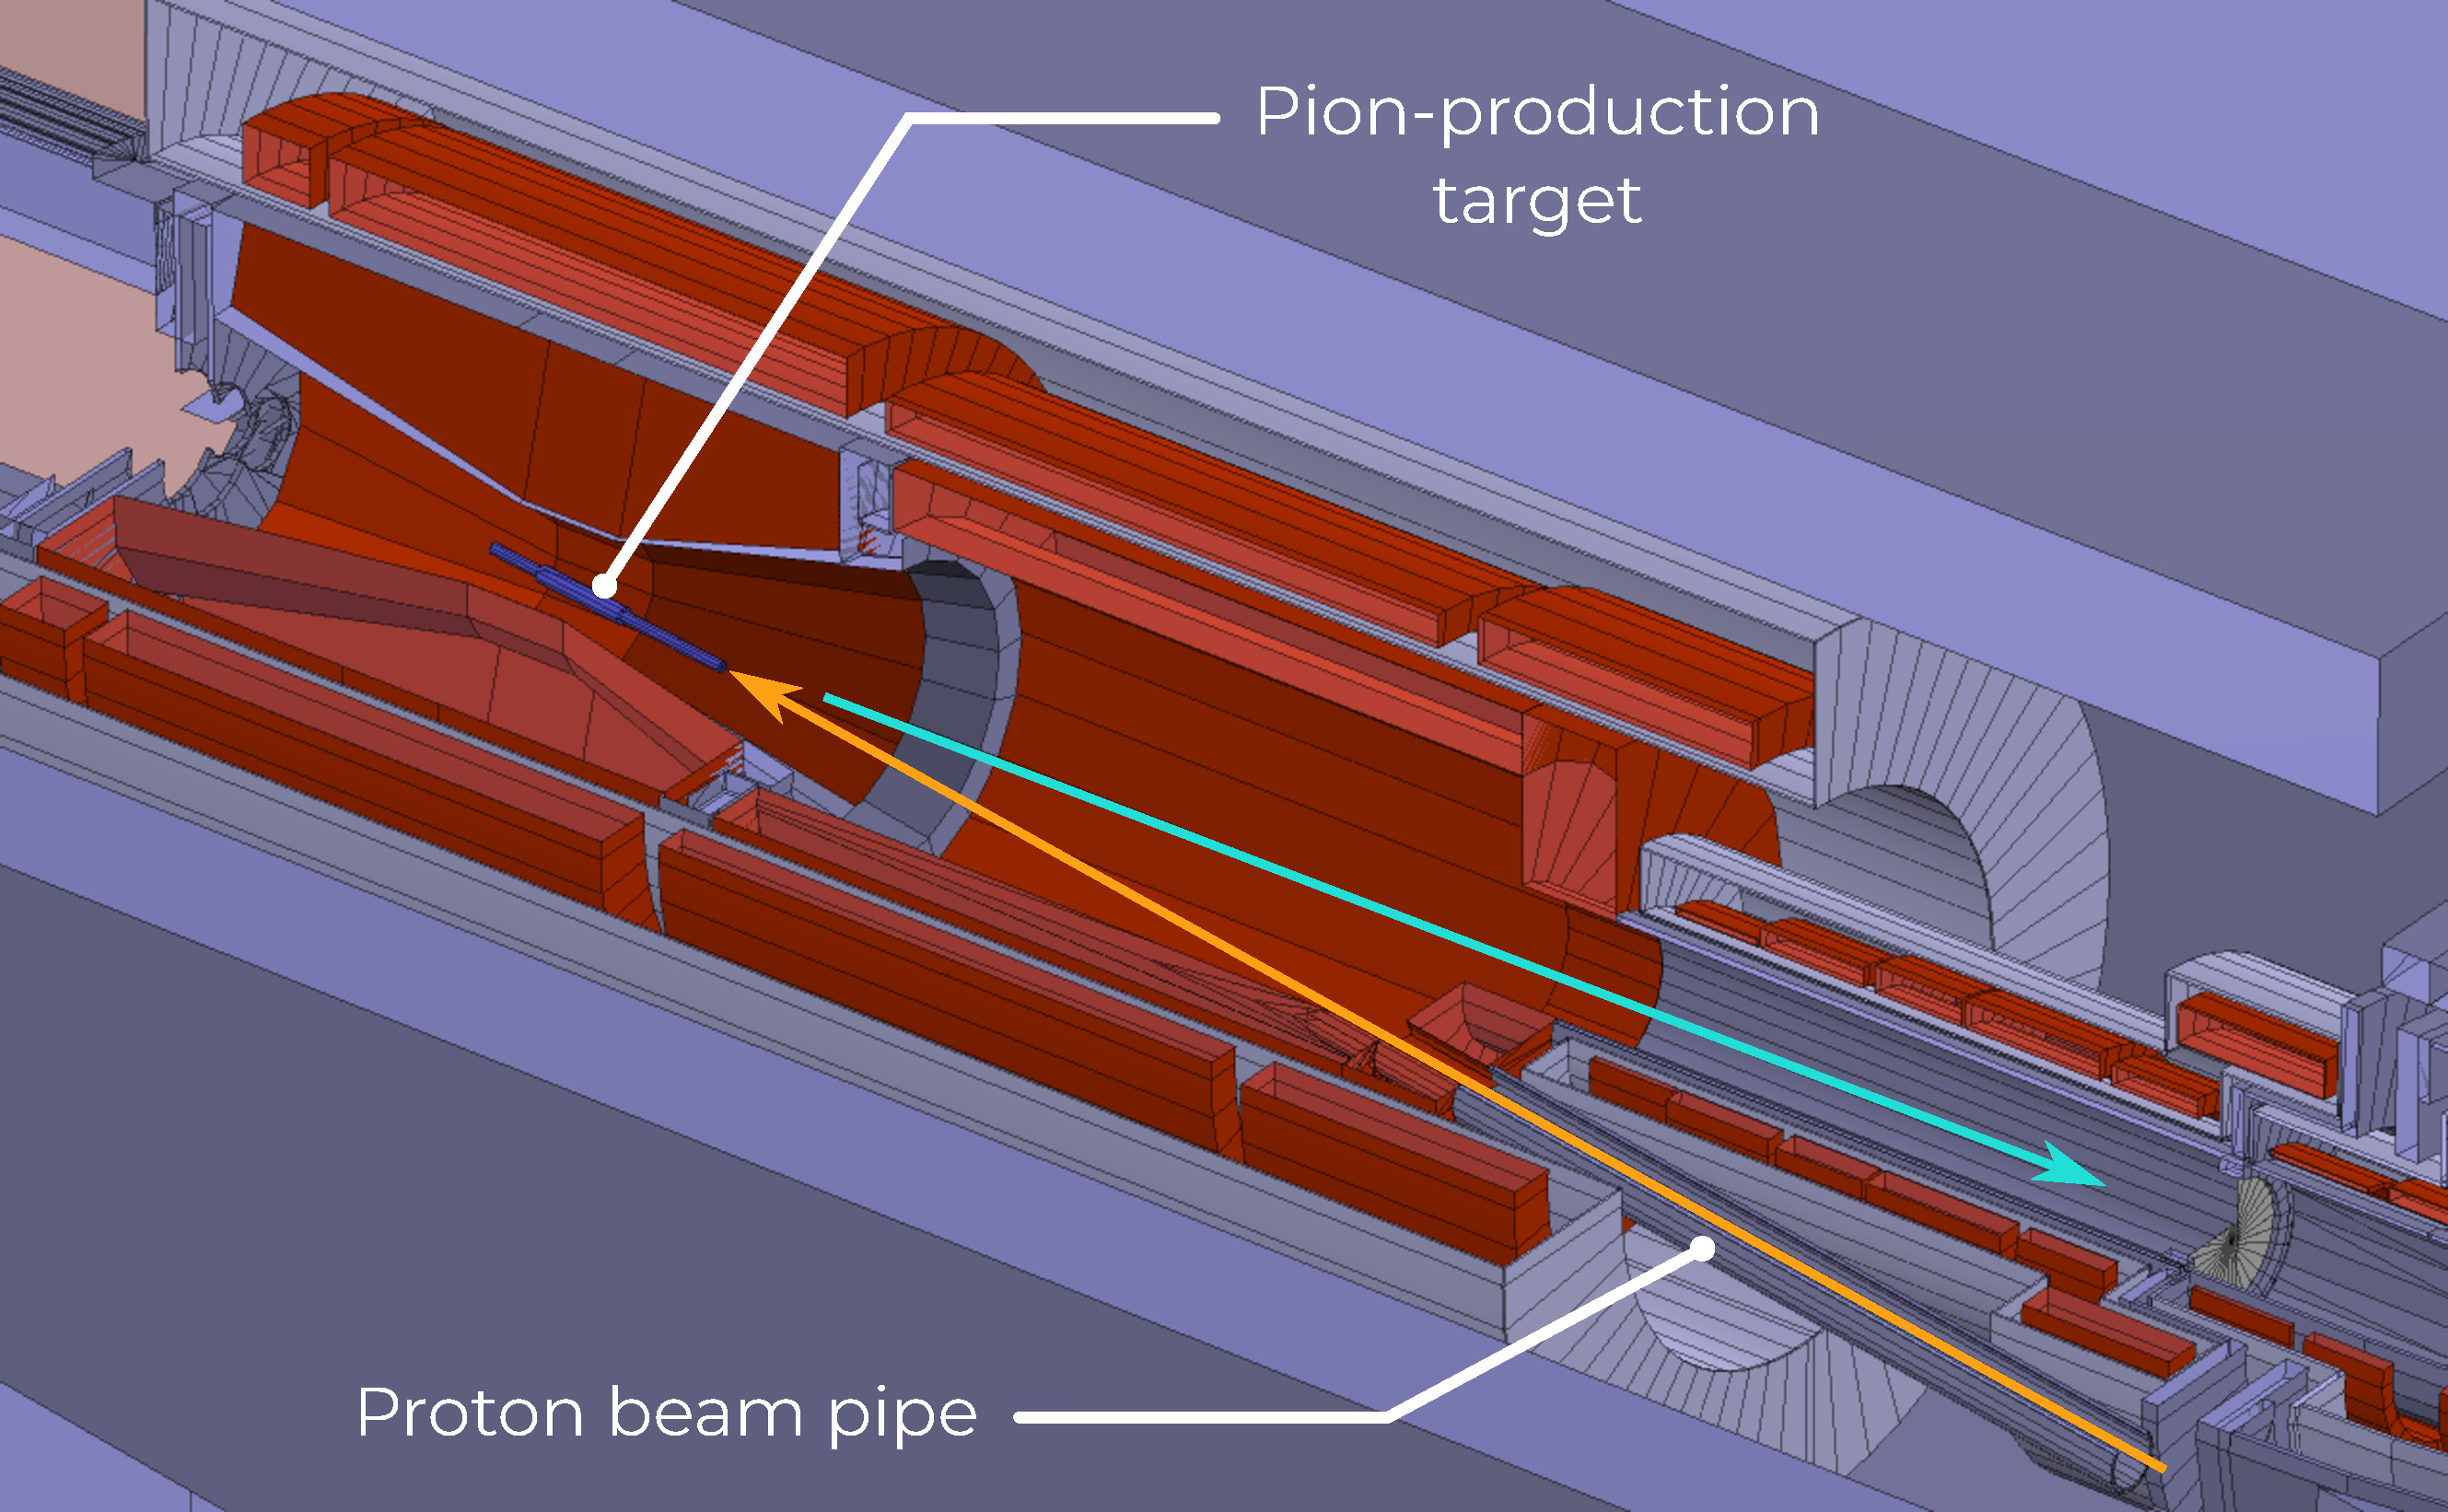
\includegraphics[width=0.8\textwidth]{chapter2/pion_production_section.png.pdf}
    \caption{ Cutaway view of the pion-production section. The orange arrow
        indicates the path of the proton beam while the teal arrow shows the
        direction of backward-going pions captured by the magnetic field.}
    \label{fig:pion_production_section}
\end{figure}

Pions are produced by the collision of the proton beam on a solid target made of
graphite in Phase-I, and tungsten in Phase-II. This region is permeated by a
\SI{5}{\tesla} magnetic field generated by a superconducting solenoid, which
confines the pions and directs them toward the transport solenoid.
Figure~\ref{fig:pion_production_section} shows a cutaway view of this
region.


Pions produced moving backward with respect to the proton beam have a lower
energy than those produced going forward, although they are not as numerous. In
COMET, it is crucial to eliminate high-energy particles in the muon beam that
could produce secondaries mimicking the conversion signal. Hence, the beamline
is positioned in the opposite direction to the proton beam such that only those
low-energy backward-moving pions are allowed into the COMET beamline.
Figure~\ref{fig:pion_momentum} illustrates this by showing that pions moving
backward with respect to the proton beam have a much lower momentum cut-off than
forward-moving pions.

\begin{figure}
    \centering
    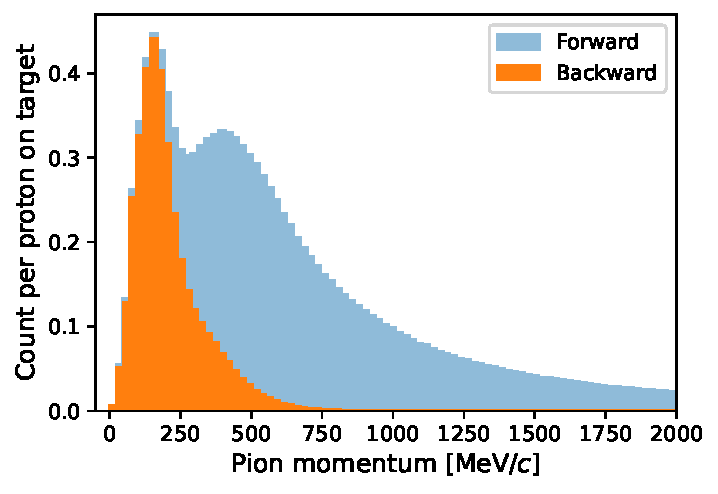
\includegraphics[width=0.5\textwidth]{chapter2/pion_mom-v2.pdf}
    \caption{ Momentum distribution of pions produced by simulating proton
    collisions with Geant4, depending on whether their initial direction is
    forward or backward with respect to the proton beam direction. }
    \label{fig:pion_momentum}
\end{figure}

\section{Transport solenoid}\label{sec:curved_solenoids}

\begin{figure}
    \centering
    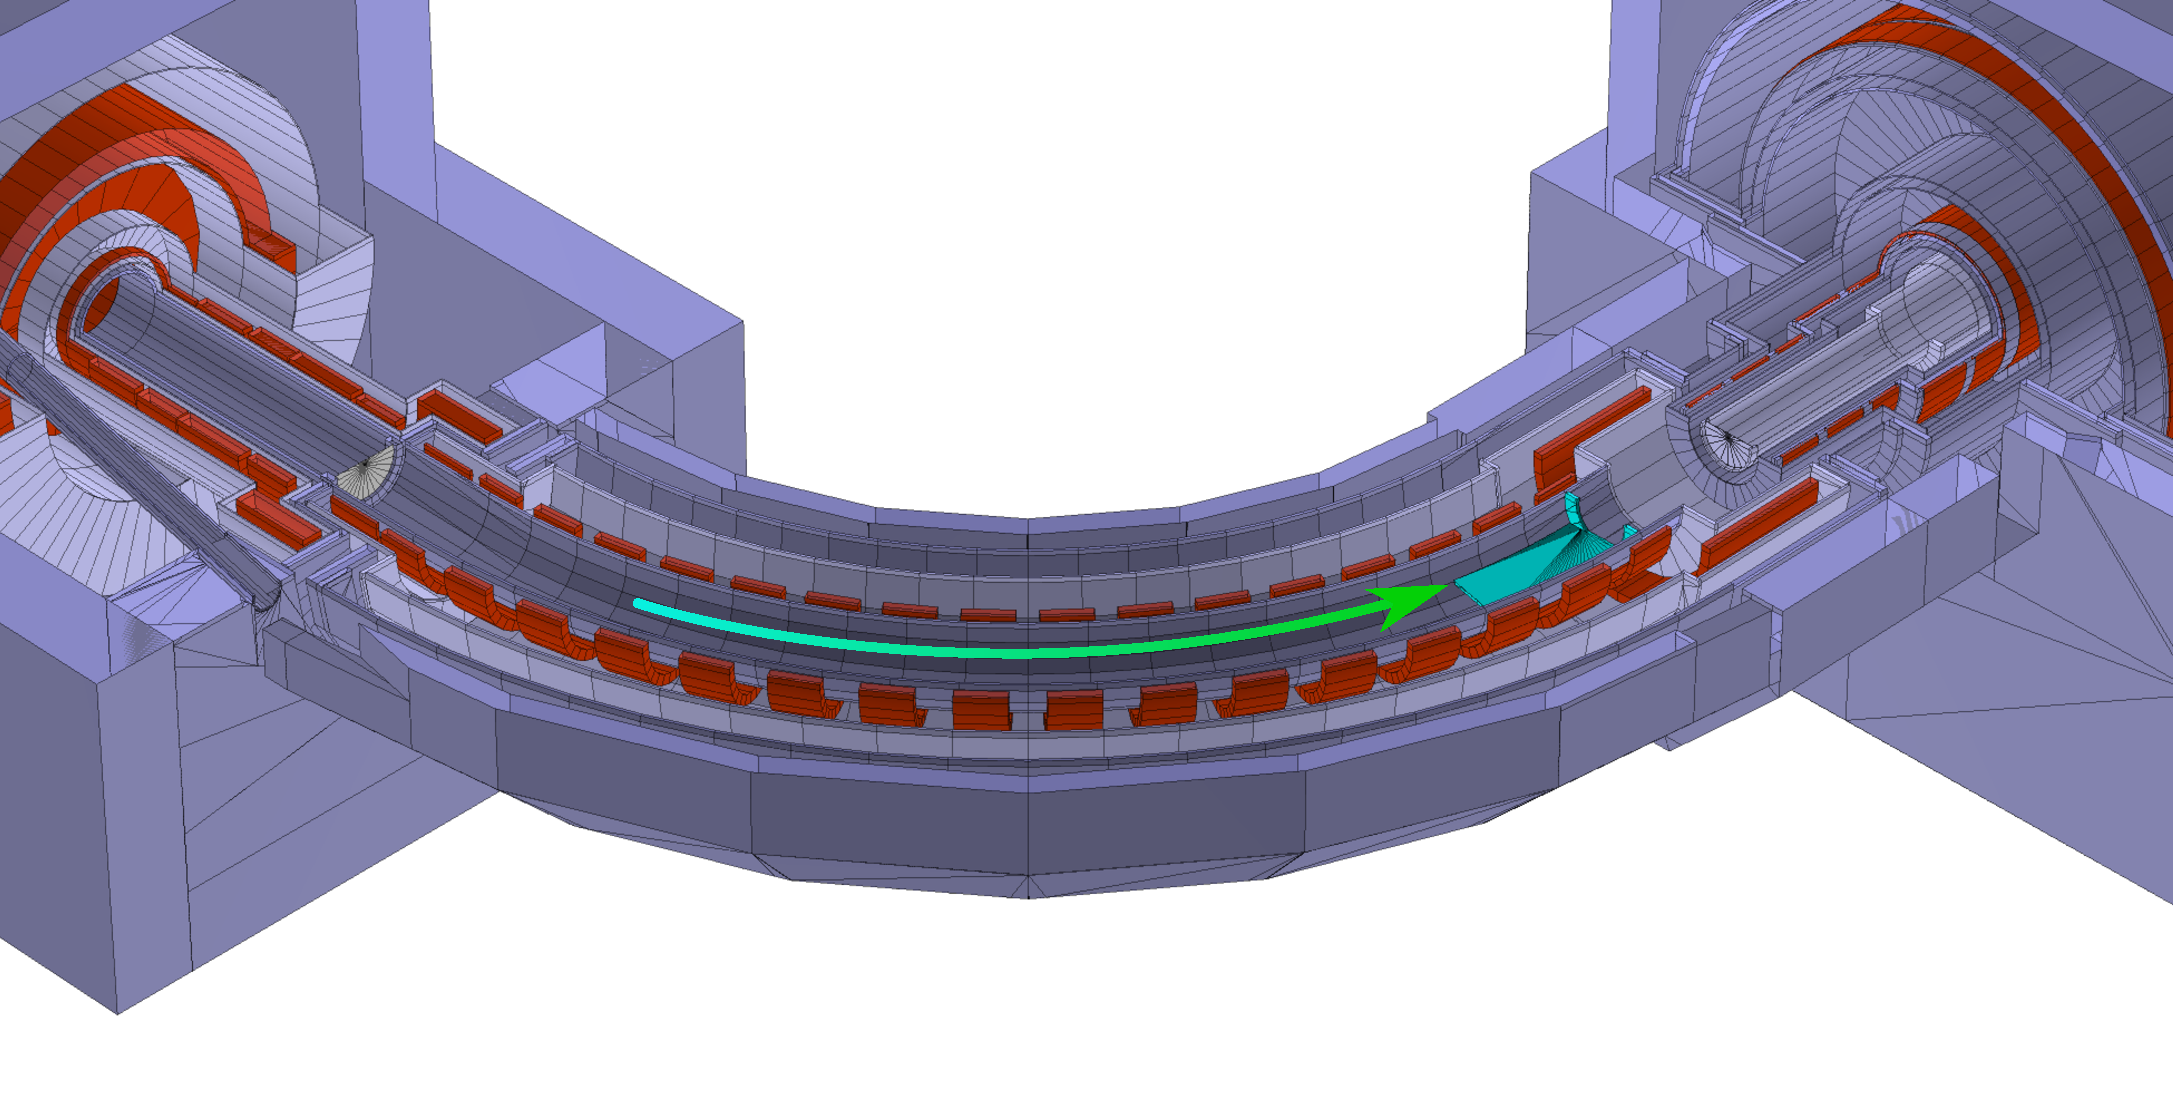
\includegraphics[width=0.8\textwidth]{chapter2/transport_solenoid.pdf}
    \caption{ Cutaway view of the Phase-I transport solenoid. The curved
        solenoid (in red) combined with collimators (in teal) select particles
        depending on their charge and momentum. }
    \label{fig:transport_solenoid}
\end{figure}

The transport solenoid is a curved pipe connecting the pion-production section
to the muon stopping section. Its purpose is twofold. Firstly, it allows a
larger fraction of pions to decay along the length of the beamline. Secondly,
the curved shape combined with its magnetic field and collimators allows it to
select negatively charged particles of a specific momentum. 


The magnetic field of a curved solenoid is slightly stronger on the inside of
the curve than on the outside. Since charged particles follow helical
trajectories, this has the net effect of making them drift vertically and the
amount of drift $D$ depends on momentum $p$ according to the equation
\begin{equation*}
    D = \frac{1}{q B} \frac{s}{R} \frac{2 p^2_L + p^2_T}{2 p_L},
\end{equation*}
where $q$ is the charge, $B$ is the strength of the field along the gyration
axis, $s$ is the distance travelled along the solenoid, $R$ is the radius of the
curve, and $p_L$ and $p_T$ respectively denote momentum longitudinal and
transverse to the solenoid axis~\cite{ben_thesis}. From this expression, one can
see that oppositely charged particles drift in opposite directions, and that
drift is overall stronger for higher-momentum particles. The ratio
$\frac{p_L}{p_T}$, which defines a helical trajectory's \emph{pitch angle}, is
also a major factor in a particle's drift.

\begin{figure}
    \centering
    \begin{subfigure}[b]{0.46\textwidth}
        \centering
        \hspace{-0.8cm}
        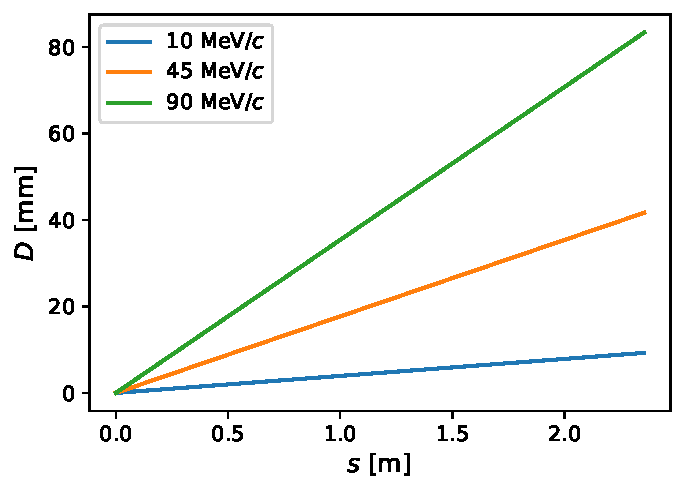
\includegraphics[width=\textwidth]{chapter2/drift_vs_s_0mT.pdf}
        \caption{No dipole field.}
    \end{subfigure}
    \hfill
    \begin{subfigure}[b]{0.46\textwidth}
        \centering
        \hspace{-0.8cm}
        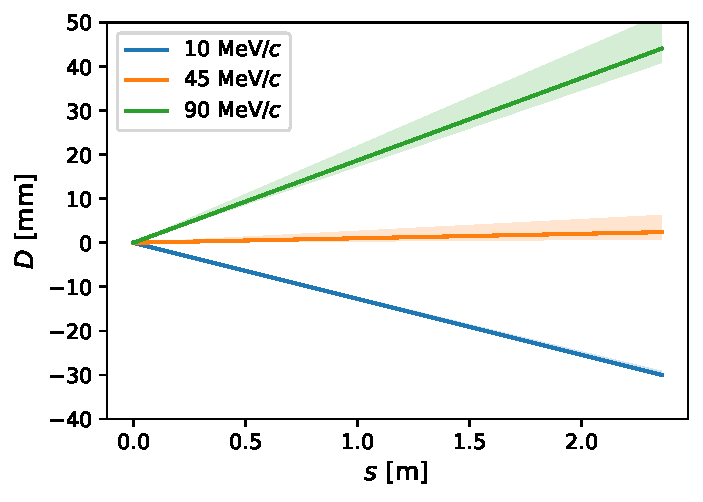
\includegraphics[width=\textwidth]{chapter2/drift_vs_s_0.05mT.pdf}
        \caption{\SI{0.05}{\tesla} vertical dipole field.}
    \end{subfigure}
    \caption{ Effective drift of particles of various momenta as they progress
        along the Phase-I transport solenoid. Solid lines show drift for a pitch
        angle of \SI{45}{\degree}, and the surrounding bands show the effect of
        a $\pm \SI{10}{\degree}$ change in pitch angle on the drift. By applying
        an additional vertical magnetic field, particles of a specific momentum
        can be selected. Here, a \SI{0.05}{\tesla} dipole field allows
        particles around \SI{45}{\MeV/\clight} to stay on axis while higher- and
        lower-momentum particles drift in opposite directions, and can then be
        suppressed by collimators at the end of the transport section. }
    \label{fig:drift}
\end{figure}

The drift caused by the curved solenoid makes all particles of the same charge
move in the same direction to varying degrees depending on momentum. In order to
select particles of a specific momentum, a vertical component is added to the
magnetic field to counterbalance the drift. Selected particles thus stay on
axis, while higher- and lower-momentum particles drift off axis. With the addition
of a collimator at the end of the transport solenoid, particles with unwanted
momenta are effectively eliminated from the beam.

Figure~\ref{fig:drift} shows drift $D$ as a function of $s$, the longitudinal
distance travelled by particles along the solenoid. This illustrates how, by
adding a dipole field, particles with a momentum outside the required range can
be efficiently eliminated by collimators at the top and bottom of the beam pipe.

\section{Muon stopping target}\label{sec:stopping_target}
The purpose of the muon stopping target is to slow down and stop as many muons
as possible while not blocking the path of converted electrons. It is composed
of a series of 17 thin aluminium disks placed in the way of the muon beam. The
disks are \SI{20}{\cm} in diameter, \SI{0.2}{\mm} thick, and separated by
\SI{5}{\cm}. The stopping target is shown in Figure~\ref{fig:cydet}, surrounded
by the Cylindrical Detector.

The more aluminium there is, the higher the number of muons that will be stopped
and allowed to undergo conversion. However, more material also means more energy
lost by electrons flying outward, hence the design of the target optimises
between muon stopping rate and acceptance of conversion electrons by the
detector system.


The material of the stopping target influences the conversion rate, but also the
lifetime of a muon caught in orbit around a nucleus. A heavy target favours the
expected rate of $\mu$--$e$ conversion, however it also causes the nuclear
capture rate to be higher. In COMET, beam bunches are separated by
\SI{1.17}{\ns} and prompt backgrounds typically die off within a few hundred
nanoseconds. A muonic atom with an iron or heavier nucleus has a lifetime less
than \SI{200}{\ns}~\cite{ben_thesis}, which would be too short to allow muons to
stay bound and convert after the beam flash is over. Hence, a light target such
as aluminium, with a longer stopped muon lifetime of
\SI{864}{\ns}~\cite{PhysRevC.35.2212}, is better suited to the COMET conversion
search.

\section{Detector systems}
\subsection{StrECAL}


\begin{figure}
    \centering
    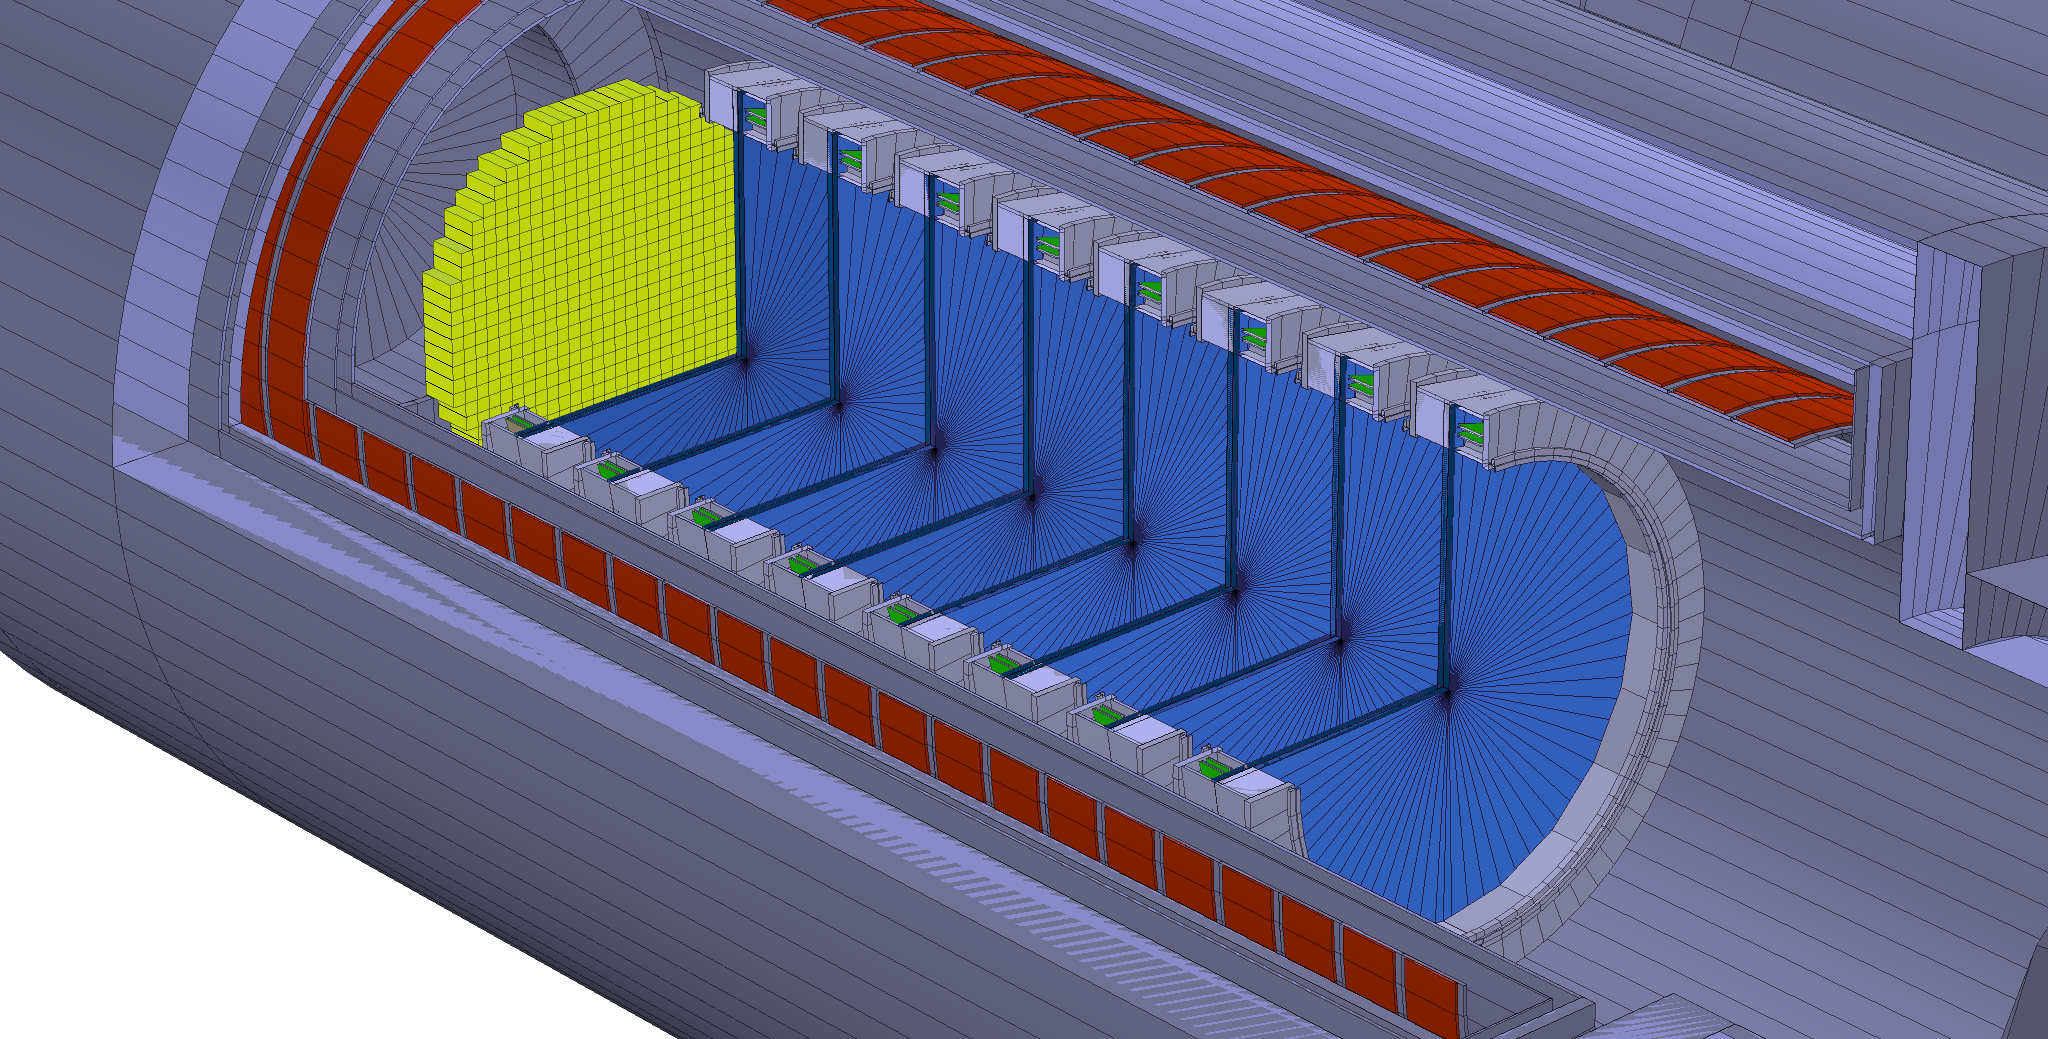
\includegraphics[width=0.8\textwidth]{chapter2/strecal_recolor.png}
    \caption{ Cutaway view of the StrECAL detector. The Straw Tracker stations
    are shown in blue and the ECAL in yellow.  }
    \label{fig:strecal}
\end{figure}

The StrECAL combines a straw-tube tracking detector with an electromagnetic
calorimeter for energy measurement. In COMET Phase-I, the StrECAL will serve as
a beam characterisation apparatus. It will be placed directly at the end of the
transport solenoid, without a muon stopping target, to study the composition of
the COMET beam and gain a more thorough understanding of potential backgrounds.
The collected data can also serve to validate and refine the Monte Carlo
simulation in preparation for the conversion measurement.

In COMET Phase-II, the StrECAL will serve as the detector system for the
conversion measurement. It will be placed after the electron spectrometer, a
curved solenoid section designed to select conversion electrons, as shown in
Figure~\ref{fig:comet_schematic}. Figure~\ref{fig:strecal} shows a rendering of
the StrECAL detector system in Phase-II.

The Straw Tracker uses thin straw tubes as drift chambers, arranged into
circular planes. A series of stations, each one able to measure the horizontal
and vertical position of a particle, are positioned along the beam direction.
The straws have a resolution better than \SI{100}{\um}, which allows the Straw
Tracker to reconstruct trajectories and estimate particle momenta via
time-of-flight information.

The ECAL is a crystal electromagnetic calorimeter which supplements the Straw
Tracker in measuring energy and thus in identifying electrons. The ECAL uses
lutetium-yttrium oxyorthosilicate (LYSO) as its scintillating crystals and
avalanche photodiodes to collect the emitted photons.



\subsection{CyDet}

\begin{figure}
    \centering
    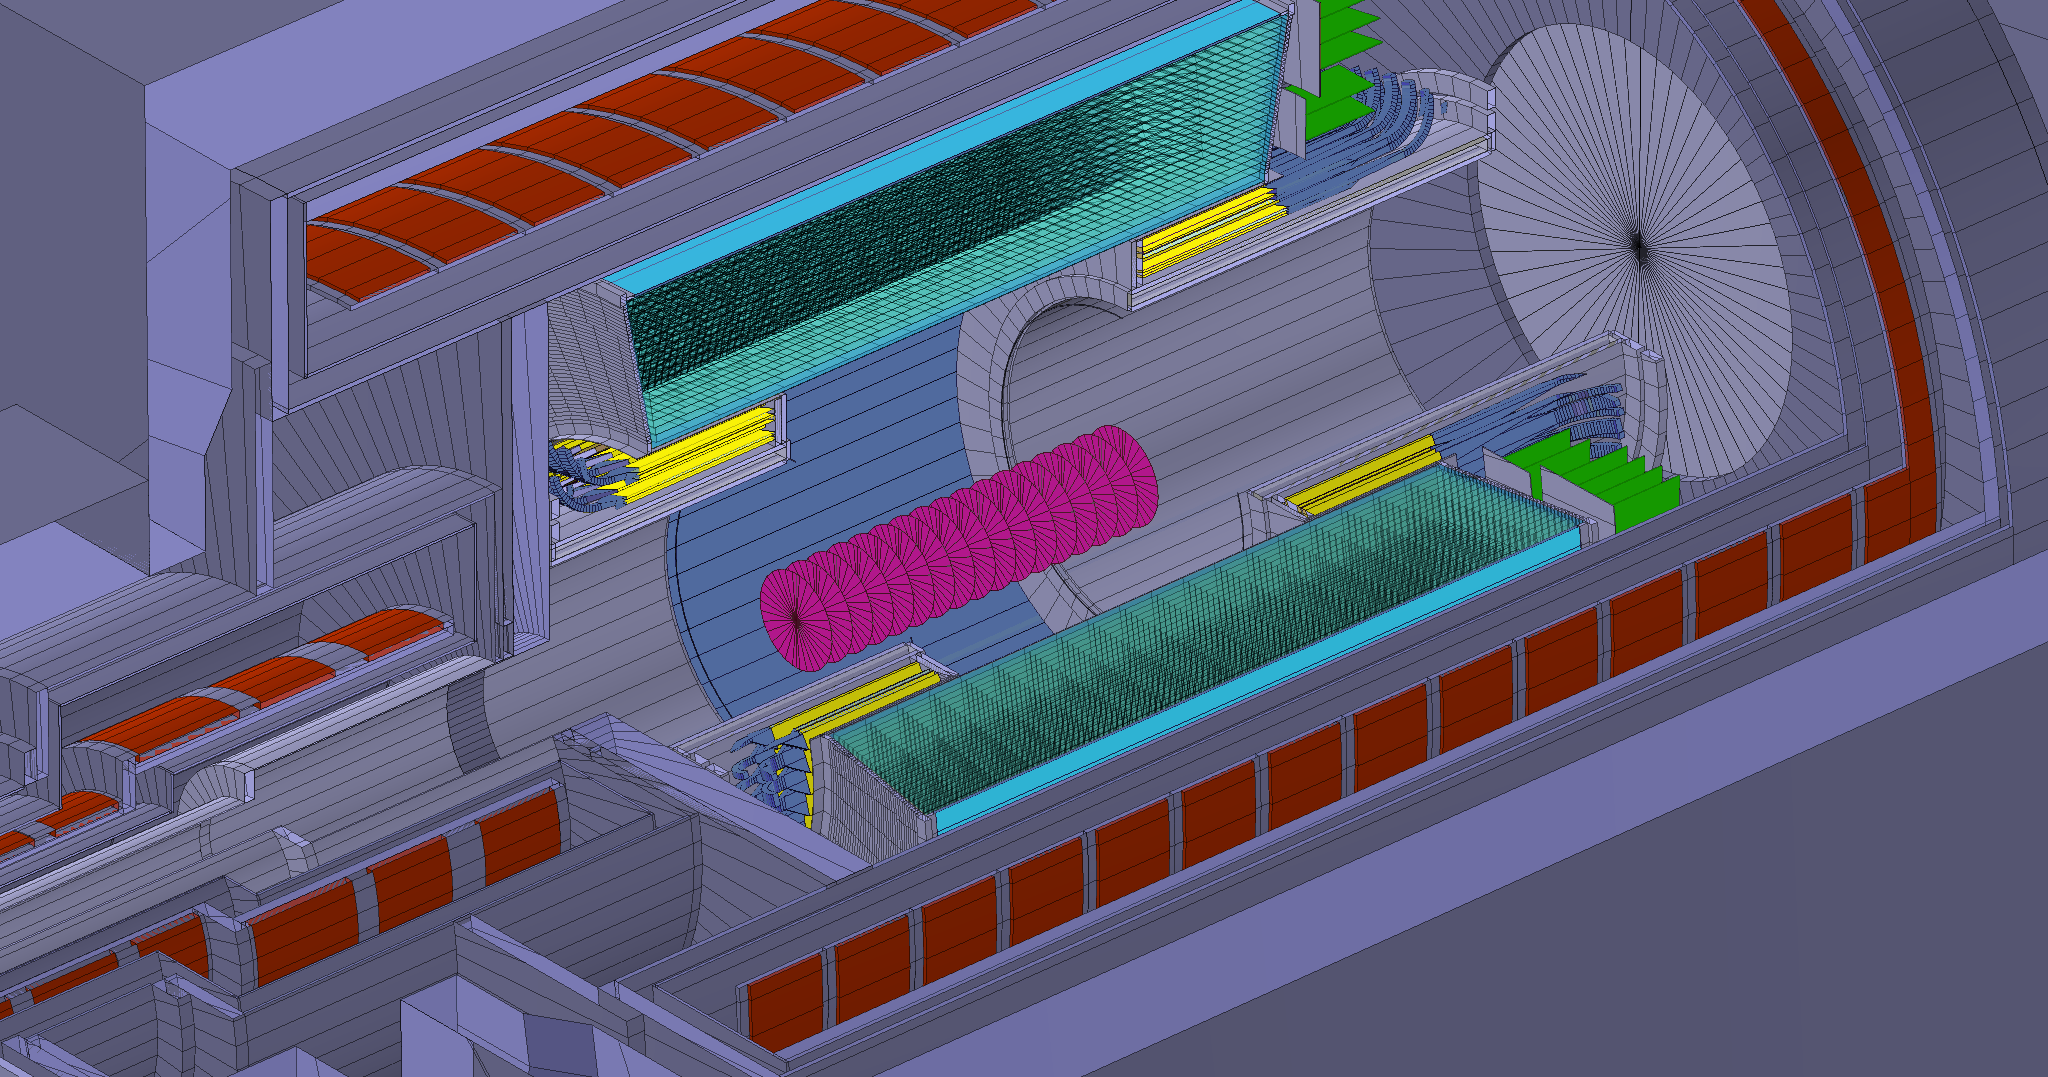
\includegraphics[width=0.8\textwidth]{chapter2/cydet_recolor.png}
    \caption{ Cutaway view of the Cylindrical Detector, composed of the
        Cylindrical Drift Chamber (in teal) and Cylindrical Trigger Hodoscope
        (in yellow). The muon stopping target disks, in purple, sit in the
        centre of the detector system. }
    \label{fig:cydet}
\end{figure}

The Cylindrical Detector (CyDet) consists of a Cylindrical Drift Chamber (CDC)
for tracking and a Cylindrical Trigger Hodoscope (CTH) for triggering on
specific event signatures. The CyDet surrounds the muon stopping target and sits
within the detector solenoid which generates a \SI{1}{\tesla} longitudinal
magnetic field. This configuration, shown in Figure~\ref{fig:cydet}, is designed
to eliminate backgrounds from the beam itself as well as low-momentum products
of the collision while maximising the acceptance of conversion electrons.
Figure~\ref{fig:cydet_signal_event} additionally shows the signature of a
simulated conversion electron inside the CyDet system.


\subsubsection{Cylindrical Drift Chamber}
The CDC is a drift chamber used to track charged particles emanating from the
muon stopping target. In order to suppress hits from beam particles, the CDC is
wrapped around the beam pipe and has an inner radius of \SI{50}{\cm}. Combined
with the \SI{1}{\tesla} longitudinal magnetic field, this prevents charged
particles with a transverse momentum less than \SI{60}{\MeV/\clight} from
reaching the chamber. In order to achieve the sensitivity goal for Phase-I, the
CDC has a momentum resolution better than \SI{200}{\keV/\clight} in order to
differentiate between conversion electrons and electrons from the high-energy
tails of the decay-in-orbit and radiative muon capture spectra. 

% Geometry
The CDC contains 4986 \emph{sense wires} strung out longitudinally in 20
concentric layers. The wires in each layer are rotated slightly off of the
longitudinal axis, and the rotation is alternatively clockwise and
anti-clockwise from one layer to the next. This special property, called the
\emph{stereo angle}, allows the drift chamber to stereoscopically reconstruct,
within \SI{3}{\mm}, the longitudinal position of a particle~\cite{ewen_thesis}. 


% Operating principle
Each sense wire is held at a potential of up to \SI{1900}{\volt} and is
surrounded by 8 grounded \emph{field wires} to generate an inward electric
field. When a charged particle ionises the gas, the field accelerates freed
electrons toward the sense wire. These electrons can gain enough energy to further
ionise the gas, leading to avalanche multiplication (see
e.g.~\cite[Chapter~6]{leo}). The avalanche produces a pulse on the sense wire,
which is acquired by the readout electronics. 


% Drift time

% The time period between the passage of the ionising charged particle and the
% ionisation products inducing a pulse on the wire depends on the \emph{drift
% velocity} of the gas, which depends on the applied voltage.

% ... not necessary?

\subsubsection{Cylindrical Trigger Hodoscope}
The CTH consists of two \emph{modules} that line the inner wall of the CDC, one
upstream and one downstream of the muon stopping target. Each module contains
two layers of 48 partially-overlapping scintillation counters. Each counter has
a time resolution of \SI{1}{\ns}. The main purpose of the CTH is to reject
background events coming from the beam itself and from products of the muon beam
collision while complementing the CDC in identifying conversion electrons.

The overlap between counters allows the CTH to reject a large fraction of
background hits, e.g.\ from photons produced in the muon beam collision. This is
done by only accepting fourfold-coincident events, where four neighbouring
counters (two in the inner layer, two in the outer layer) are hit in a short
\SI{10}{\ns} time span. The CTH thus provides an online triggering mechanism
which significantly reduces the number of background events accepted by the
CyDet system due to its proximity with the muon stopping target.
Figure~\ref{fig:cydet_signal_event} shows how a conversion electron might
produce such a fourfold coincidence.


\subsection{Cosmic ray veto}
\label{sec:crv}
The COMET experiment hall is constantly irradiated by muons produced in the
atmosphere by cosmic rays. The cosmic ray veto (CRV) is an additional active
detector which will tightly enclose the CyDet and StrECAL detector systems. Its
purpose is to identify events induced by atmospheric muons rather than by the
COMET beam, and thus reduce the probability that such events will be mistaken
for a conversion signal.

\section{Conversion signature}
Conversion electrons are mono-energetic at $E=\SI{104.97}{\MeV}$ and emitted
isotropically by muons stopped in the target disks. In the magnetic field of the
detector solenoid, they have a helical trajectory which can be reconstructed by
the CDC or Straw Tracker. Figure~\ref{fig:cydet_signal_event} shows a simulated
conversion electron going through the Cylindrical Detector.



\begin{figure}
    \centering
    %\captionsetup[subfigure]{justification=centering}
    \begin{subfigure}[b]{0.43\textwidth}
    \centering
    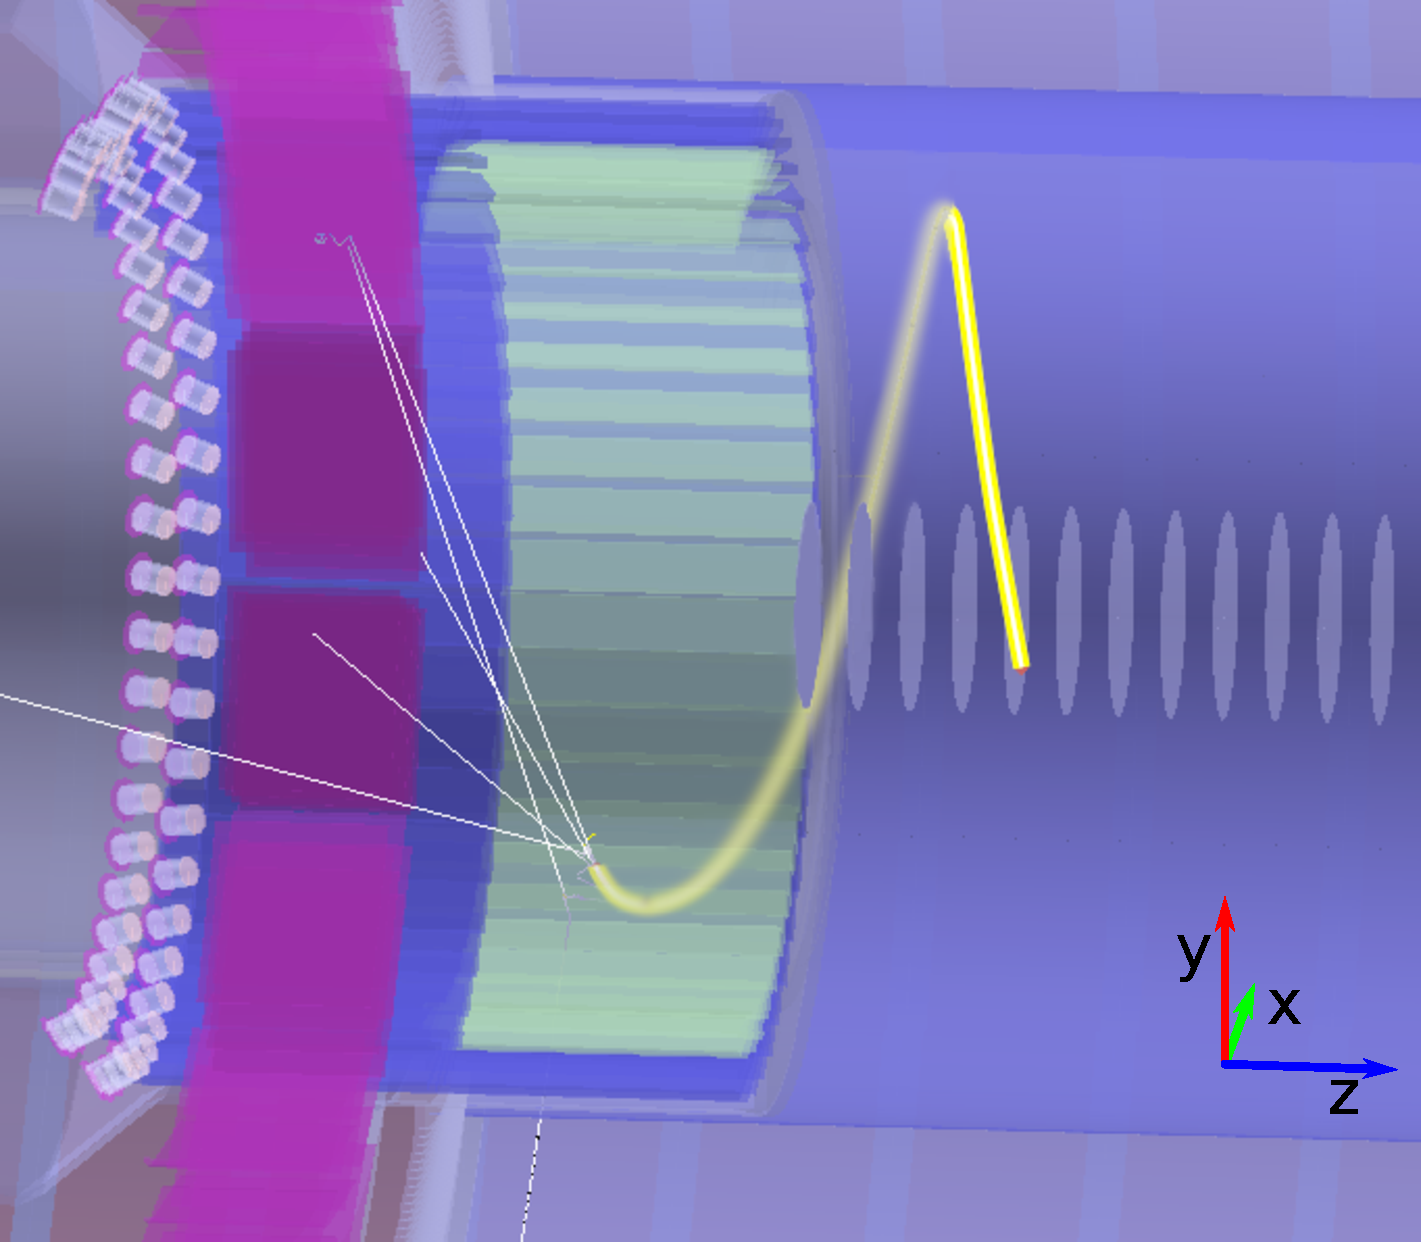
\includegraphics[width=0.85\textwidth]{chapter2/signal_event_display_crop_axes.pdf}
    \vspace{1.18cm}
    \caption{Event shown in \texttt{DisplayCore}, the 3D event display of
    ICEDUST (see Chapter~\ref{ch:software}).}
    \end{subfigure}
    \hfill
    \begin{subfigure}[b]{0.53\textwidth}
    \centering
    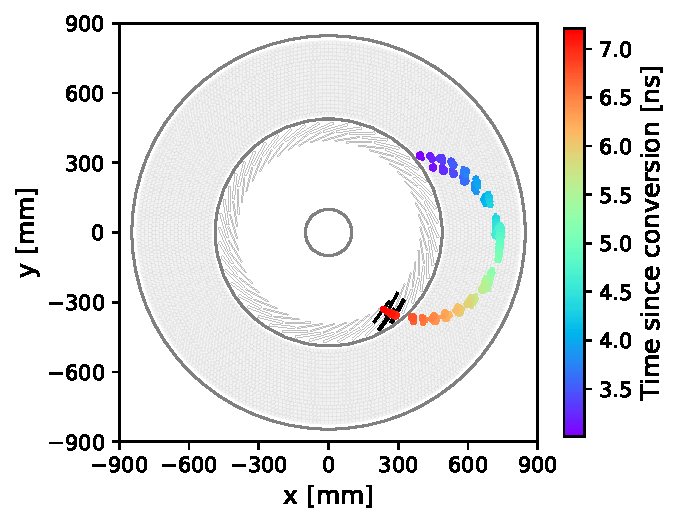
\includegraphics[width=0.99\textwidth]{chapter2/cydet_signal_track_v4.pdf}
    \caption{CyDet event display showing the timing of hits since conversion.}
    \end{subfigure}
    
    \caption{ Conversion electron trajectory as observed by the Cylindrical
    Detector. The effect of stereo angles is visible at the start of the
    trajectory where hits have alternating azimuthal positions around the actual
    electron track. Upon reaching the CTH, the electron produces consecutive
    hits in four adjacent counters, satisfying the fourfold coincidence trigger
    criterion.}
    \label{fig:cydet_signal_event}
\end{figure}


% Timing
The expected timing of conversion electrons is directly related to the time
distribution of muons bound inside the stopping target, shown in
Figure~\ref{fig:timing_distributions}. In Phase-I, in order to suppress prompt
backgrounds from the beam flash, the detector is tuned to only start triggering
on events that occur at least $t=\SI{700}{\ns}$ after each proton collision.
This acceptance criterion retains only \SI{30}{\percent} of all signal events
because the majority of bound muons, having an average lifetime of \SI{864}{\ns},
will have undergone decay or capture before the start of the window.


\section{Experimental backgrounds}\label{sec:backgrounds}

\begin{table}
    \centering
    \begin{tabular}{l|cccc|c}
        \toprule
        Background source & Intrinsic & Stray protons & Antiprotons &
        Cosmics  & Total\\ 
        Estimated events & 0.014 & 0.007 & 0.001 & 0.010 & 0.032 \\ \bottomrule
    \end{tabular}
    \caption{Expected number of background events from each potential
    source~\cite{the_comet_collaboration_comet_2020}. The total count is much
    smaller than one, such that the observation of a single signal electron
    could be evidence that charged lepton flavour is violated.}
    \label{tab:backgrounds}
\end{table}

Intrinsic backgrounds from muon decay-in-orbit and nuclear muon capture can
mimic the conversion signal, as discussed in Section~\ref{sec:sm_backgrounds}.
The COMET experiment is also affected by experimental backgrounds caused by the
intense beam, as well as cosmic ray-induced events.

Beam-induced backgrounds include delayed events caused by slow particles and
products of stray protons arriving between two bunches.
Antiprotons are the main source of delayed backgrounds due to their slow
speed relative to pions and muons of the same momentum. They are negatively
charged so cannot be efficiently selected out by the beamline, hence they can
collide late with the muon stopping target and produce signal-like secondary
electrons during the trigger window.

When a stray proton hits the pion-production target late, secondaries may
quickly travel to the detector region and produce a signal-like electron, which
can also be mistaken for the conversion signal. This is the main reason for
requiring the strict extinction factor $R_\mathrm{extinction}$ of
Equation~\ref{eq:extinction} from the J-PARC proton beam.

Finally, cosmic rays could be a major source of background events. The
background rate depends heavily on the amount of shielding and material above
the COMET detector system, as well as the efficiency of the cosmic ray veto. The
topic of rate estimation for cosmic ray-induced backgrounds is discussed more
thoroughly in Chapter~\ref{ch:cosmics}.



Table~\ref{tab:backgrounds} shows the rates estimated in the COMET Phase-I
technical design report (TDR)~\cite[Section
10.6]{the_comet_collaboration_comet_2020} for each source of background in the
$\mu$--$e$ conversion search. The total number of background events over the
data acquisition run time is predicted to be 0.032 given an extinction factor
$R_\mathrm{extinction} = 3 \times 10^{-11}$. Since this background event count
is much smaller than one, the observation of a single signal-like electron may
suggest that a CLFV process is at play, which would further motivate this search
through COMET Phase-II and beyond.



% Backgrounds = signal contamination. Backgrounds do not enter the equation for
% SES, but SES involves quality cut factors whose purpose is to lower background
% rates. The goal is to show that background rate << 1, only then SES makes
% sense since we've shown that we can actually detect a single event with little
% doubt that it's a conversion signal.


\section{Sensitivity and run time}\label{sec:SES}

The sensitivity of the COMET experiment is conventionally expressed as a
\emph{single event sensitivity} (SES), which is defined as the value of the
$\mu$--$e$ conversion branching ratio for which COMET expects to observe one
event (smaller is better). SES takes into account the net acceptance of signal events by the
detector system, however it does not say anything about the experimental
backgrounds. When using SES as a figure of merit, a study of potential
background sources is usually necessary to show that the expected number of
background events is not greater than one. 

The total number of coherent $\mu$--$e$ conversions produced by a
population of $N_\mu$ bound muons can be expressed as
$$
N_\mathrm{conversion} = N_\mu \cdot \mathcal{B}_\mathrm{conversion} \cdot
\mathcal{B}_\mathrm{capture} \cdot f_\mathrm{coherent},
$$
where $\mathcal{B}_\mathrm{conversion}$ is the conversion branching ratio
normalised to the branching ratio of nuclear muon capture
$\mathcal{B}_\mathrm{capture}$, and $f_\mathrm{coherent}$ is the fraction of
conversions estimated to occur coherently and leave the nucleus in its ground
state.
The number of conversion electrons that will be observed by the detector is then
$N_\mathrm{obs} = N_\mathrm{conversion}\, A_{\mu-e}$, where $A_{\mu-e}$ is the
detector's net signal acceptance. If we require $N_\mathrm{obs} = 1$ and
rearrange to find the corresponding value of $\mathcal{B}_\mathrm{conversion}$,
we obtain the single event sensitivity:
\begin{equation}\label{eq:ses}
\mathrm{SES} \, \equiv \, \mathcal{B}_\mathrm{conversion}^{N_\mathrm{obs}=1}
 = \, \frac{1}{N_\mu \  A_{\mu-e} \  
\mathcal{B}_\mathrm{capture} \  f_\mathrm{coherent}}.
\end{equation}
In COMET Phase-I, the signal acceptance can be broken down into seven efficiency
factors: geometrical acceptance, hardware (trigger and data acquisition), track finding,
track reconstruction quality cuts, momentum window and trigger time window.
Table~\ref{tab:acceptance} lists these factors as they were estimated in the
COMET Phase-I TDR~\cite[Section 10.1]{the_comet_collaboration_comet_2020}. 

\begin{table}
    \centering
    \begin{adjustbox}{max width=1.1\textwidth,center}
    \begin{tabular}{l|cccccc|c}
        \toprule
        Factor & Geometrical & Hardware & Track-finding & Cuts & Momentum
        & Timing & Net
        \\ 
        Efficiency & \SI{26}{\percent} & \SI{81}{\percent} &
        \SI{99}{\percent} & \SI{70}{\percent} & \SI{93}{\percent} &
        \SI{30}{\percent} & \SI{4.1}{\percent} \\
        \bottomrule
    \end{tabular}
    \end{adjustbox}
    \caption{ Efficiency factors used to determine the signal acceptance in the
    COMET Phase-I TDR~\cite{the_comet_collaboration_comet_2020}. The net
    acceptance is the product of all efficiency factors. ``Cuts'' refers to
    track quality cuts, used to reject events with irregular tracks that cannot
    be accurately fitted and reconstructed.}
    \label{tab:acceptance} 
\end{table}

From the net signal acceptance $A_{\mu-e} = \SI{4.1}{\percent}$, we can now
estimate the total data acquisition run time required to reach the sensitivity
goal of the experiment, $\mathrm{SES} = 3\times 10^{-15}$, using
Equation~\ref{eq:ses}. The required number of bound muons is thus $N_\mu = 1.5
\times 10^{16}$. This quantity can be related to the total run time $T$ via the
proton beam current $I_p = \SI{0.4}{\micro\ampere}$ and the yield of stopped
muons per collision $R_{\mu / p} = 4.7\times 10^{-4}$:
$$
N_\mu = T \cdot \frac{I_p}{e} \cdot R_{\mu / p}.
$$
This equation is rearranged for $T$ to yield $T = 146$~days of data acquisition
for a Phase-I SES of $3 \times 10^{-15}$.
